% Options for packages loaded elsewhere
\PassOptionsToPackage{unicode}{hyperref}
\PassOptionsToPackage{hyphens}{url}
%
\documentclass[
]{article}
\usepackage{amsmath,amssymb}
\usepackage{lmodern}
\usepackage{iftex}
\ifPDFTeX
  \usepackage[T1]{fontenc}
  \usepackage[utf8]{inputenc}
  \usepackage{textcomp} % provide euro and other symbols
\else % if luatex or xetex
  \usepackage{unicode-math}
  \defaultfontfeatures{Scale=MatchLowercase}
  \defaultfontfeatures[\rmfamily]{Ligatures=TeX,Scale=1}
\fi
% Use upquote if available, for straight quotes in verbatim environments
\IfFileExists{upquote.sty}{\usepackage{upquote}}{}
\IfFileExists{microtype.sty}{% use microtype if available
  \usepackage[]{microtype}
  \UseMicrotypeSet[protrusion]{basicmath} % disable protrusion for tt fonts
}{}
\makeatletter
\@ifundefined{KOMAClassName}{% if non-KOMA class
  \IfFileExists{parskip.sty}{%
    \usepackage{parskip}
  }{% else
    \setlength{\parindent}{0pt}
    \setlength{\parskip}{6pt plus 2pt minus 1pt}}
}{% if KOMA class
  \KOMAoptions{parskip=half}}
\makeatother
\usepackage{xcolor}
\usepackage[margin=1in]{geometry}
\usepackage{color}
\usepackage{fancyvrb}
\newcommand{\VerbBar}{|}
\newcommand{\VERB}{\Verb[commandchars=\\\{\}]}
\DefineVerbatimEnvironment{Highlighting}{Verbatim}{commandchars=\\\{\}}
% Add ',fontsize=\small' for more characters per line
\usepackage{framed}
\definecolor{shadecolor}{RGB}{248,248,248}
\newenvironment{Shaded}{\begin{snugshade}}{\end{snugshade}}
\newcommand{\AlertTok}[1]{\textcolor[rgb]{0.94,0.16,0.16}{#1}}
\newcommand{\AnnotationTok}[1]{\textcolor[rgb]{0.56,0.35,0.01}{\textbf{\textit{#1}}}}
\newcommand{\AttributeTok}[1]{\textcolor[rgb]{0.77,0.63,0.00}{#1}}
\newcommand{\BaseNTok}[1]{\textcolor[rgb]{0.00,0.00,0.81}{#1}}
\newcommand{\BuiltInTok}[1]{#1}
\newcommand{\CharTok}[1]{\textcolor[rgb]{0.31,0.60,0.02}{#1}}
\newcommand{\CommentTok}[1]{\textcolor[rgb]{0.56,0.35,0.01}{\textit{#1}}}
\newcommand{\CommentVarTok}[1]{\textcolor[rgb]{0.56,0.35,0.01}{\textbf{\textit{#1}}}}
\newcommand{\ConstantTok}[1]{\textcolor[rgb]{0.00,0.00,0.00}{#1}}
\newcommand{\ControlFlowTok}[1]{\textcolor[rgb]{0.13,0.29,0.53}{\textbf{#1}}}
\newcommand{\DataTypeTok}[1]{\textcolor[rgb]{0.13,0.29,0.53}{#1}}
\newcommand{\DecValTok}[1]{\textcolor[rgb]{0.00,0.00,0.81}{#1}}
\newcommand{\DocumentationTok}[1]{\textcolor[rgb]{0.56,0.35,0.01}{\textbf{\textit{#1}}}}
\newcommand{\ErrorTok}[1]{\textcolor[rgb]{0.64,0.00,0.00}{\textbf{#1}}}
\newcommand{\ExtensionTok}[1]{#1}
\newcommand{\FloatTok}[1]{\textcolor[rgb]{0.00,0.00,0.81}{#1}}
\newcommand{\FunctionTok}[1]{\textcolor[rgb]{0.00,0.00,0.00}{#1}}
\newcommand{\ImportTok}[1]{#1}
\newcommand{\InformationTok}[1]{\textcolor[rgb]{0.56,0.35,0.01}{\textbf{\textit{#1}}}}
\newcommand{\KeywordTok}[1]{\textcolor[rgb]{0.13,0.29,0.53}{\textbf{#1}}}
\newcommand{\NormalTok}[1]{#1}
\newcommand{\OperatorTok}[1]{\textcolor[rgb]{0.81,0.36,0.00}{\textbf{#1}}}
\newcommand{\OtherTok}[1]{\textcolor[rgb]{0.56,0.35,0.01}{#1}}
\newcommand{\PreprocessorTok}[1]{\textcolor[rgb]{0.56,0.35,0.01}{\textit{#1}}}
\newcommand{\RegionMarkerTok}[1]{#1}
\newcommand{\SpecialCharTok}[1]{\textcolor[rgb]{0.00,0.00,0.00}{#1}}
\newcommand{\SpecialStringTok}[1]{\textcolor[rgb]{0.31,0.60,0.02}{#1}}
\newcommand{\StringTok}[1]{\textcolor[rgb]{0.31,0.60,0.02}{#1}}
\newcommand{\VariableTok}[1]{\textcolor[rgb]{0.00,0.00,0.00}{#1}}
\newcommand{\VerbatimStringTok}[1]{\textcolor[rgb]{0.31,0.60,0.02}{#1}}
\newcommand{\WarningTok}[1]{\textcolor[rgb]{0.56,0.35,0.01}{\textbf{\textit{#1}}}}
\usepackage{graphicx}
\makeatletter
\def\maxwidth{\ifdim\Gin@nat@width>\linewidth\linewidth\else\Gin@nat@width\fi}
\def\maxheight{\ifdim\Gin@nat@height>\textheight\textheight\else\Gin@nat@height\fi}
\makeatother
% Scale images if necessary, so that they will not overflow the page
% margins by default, and it is still possible to overwrite the defaults
% using explicit options in \includegraphics[width, height, ...]{}
\setkeys{Gin}{width=\maxwidth,height=\maxheight,keepaspectratio}
% Set default figure placement to htbp
\makeatletter
\def\fps@figure{htbp}
\makeatother
\setlength{\emergencystretch}{3em} % prevent overfull lines
\providecommand{\tightlist}{%
  \setlength{\itemsep}{0pt}\setlength{\parskip}{0pt}}
\setcounter{secnumdepth}{-\maxdimen} % remove section numbering
\ifLuaTeX
  \usepackage{selnolig}  % disable illegal ligatures
\fi
\IfFileExists{bookmark.sty}{\usepackage{bookmark}}{\usepackage{hyperref}}
\IfFileExists{xurl.sty}{\usepackage{xurl}}{} % add URL line breaks if available
\urlstyle{same} % disable monospaced font for URLs
\hypersetup{
  pdftitle={Untitled},
  hidelinks,
  pdfcreator={LaTeX via pandoc}}

\title{Untitled}
\author{}
\date{\vspace{-2.5em}2022-10-26}

\begin{document}
\maketitle

\includegraphics{images/paste-5183836A.png}

\begin{Shaded}
\begin{Highlighting}[]
\NormalTok{x }\OtherTok{\textless{}{-}} \StringTok{"168 161 167 179 184 166 198 187 191 179"}
\NormalTok{xi }\OtherTok{\textless{}{-}} \FunctionTok{as.numeric}\NormalTok{(}\FunctionTok{strsplit}\NormalTok{(x, }\StringTok{" "}\NormalTok{)[[}\DecValTok{1}\NormalTok{]])}
\NormalTok{x }\OtherTok{\textless{}{-}} \StringTok{"65.5 58.3 68.1 85.7 80.5 63.4 102.6 91.4 86.7 78.9"}
\NormalTok{yi }\OtherTok{\textless{}{-}} \FunctionTok{as.numeric}\NormalTok{(}\FunctionTok{strsplit}\NormalTok{(x, }\StringTok{" "}\NormalTok{)[[}\DecValTok{1}\NormalTok{]])}

\NormalTok{xbar }\OtherTok{\textless{}{-}} \FunctionTok{mean}\NormalTok{(xi)}
\NormalTok{ybar }\OtherTok{\textless{}{-}} \FunctionTok{mean}\NormalTok{(yi)}

\NormalTok{sxx }\OtherTok{\textless{}{-}} \FunctionTok{sum}\NormalTok{((xi }\SpecialCharTok{{-}}\NormalTok{ xbar)}\SpecialCharTok{\^{}}\DecValTok{2}\NormalTok{)}

\NormalTok{B1hat }\OtherTok{\textless{}{-}} \FunctionTok{sum}\NormalTok{((yi }\SpecialCharTok{{-}}\NormalTok{ ybar)}\SpecialCharTok{*}\NormalTok{(xi }\SpecialCharTok{{-}}\NormalTok{ xbar)) }\SpecialCharTok{/}\NormalTok{ sxx}
\NormalTok{B0hat }\OtherTok{\textless{}{-}}\NormalTok{ ybar }\SpecialCharTok{{-}}\NormalTok{ B1hat}\SpecialCharTok{*}\NormalTok{xbar}

\FunctionTok{print}\NormalTok{(}\FunctionTok{c}\NormalTok{(B1hat,B0hat))}
\end{Highlighting}
\end{Shaded}

\begin{verbatim}
## [1]    1.112742 -119.958107
\end{verbatim}

\includegraphics{images/paste-E37626F1.png}

\begin{Shaded}
\begin{Highlighting}[]
\NormalTok{fit }\OtherTok{\textless{}{-}} \FunctionTok{lm}\NormalTok{(yi }\SpecialCharTok{\textasciitilde{}}\NormalTok{ xi)}

\NormalTok{B0hat }\OtherTok{\textless{}{-}} \FunctionTok{coef}\NormalTok{(fit)[}\DecValTok{1}\NormalTok{]}
\NormalTok{B1hat }\OtherTok{\textless{}{-}} \FunctionTok{coef}\NormalTok{(fit)[}\DecValTok{2}\NormalTok{]}

\NormalTok{e }\OtherTok{\textless{}{-}}\NormalTok{ yi }\SpecialCharTok{{-}}\NormalTok{ (B0hat }\SpecialCharTok{+}\NormalTok{ B1hat}\SpecialCharTok{*}\NormalTok{xi)}
\NormalTok{RSS }\OtherTok{\textless{}{-}} \FunctionTok{sum}\NormalTok{(e}\SpecialCharTok{\^{}}\DecValTok{2}\NormalTok{)}
\NormalTok{n }\OtherTok{\textless{}{-}} \FunctionTok{length}\NormalTok{(xi)}
\NormalTok{df }\OtherTok{\textless{}{-}}\NormalTok{ n }\SpecialCharTok{{-}} \DecValTok{2}

\NormalTok{sigma }\OtherTok{\textless{}{-}} \FunctionTok{sqrt}\NormalTok{(RSS }\SpecialCharTok{/}\NormalTok{ (df))}
\NormalTok{sigma.B1 }\OtherTok{\textless{}{-}} \FunctionTok{sqrt}\NormalTok{( sigma}\SpecialCharTok{\^{}}\DecValTok{2}\SpecialCharTok{/}\NormalTok{sxx )}
\NormalTok{sigma.B2 }\OtherTok{\textless{}{-}} \FunctionTok{sqrt}\NormalTok{( sigma}\SpecialCharTok{\^{}}\DecValTok{2}\SpecialCharTok{/}\NormalTok{n }\SpecialCharTok{+}\NormalTok{ sigma}\SpecialCharTok{\^{}}\DecValTok{2}\SpecialCharTok{*}\NormalTok{xbar}\SpecialCharTok{\^{}}\DecValTok{2} \SpecialCharTok{/}\NormalTok{ sxx )}
\FunctionTok{c}\NormalTok{(sigma, sigma.B1, sigma.B2)}
\end{Highlighting}
\end{Shaded}

\begin{verbatim}
## [1]  3.8809005  0.1059391 18.8970518
\end{verbatim}

\includegraphics{images/paste-91FB1BDB.png}

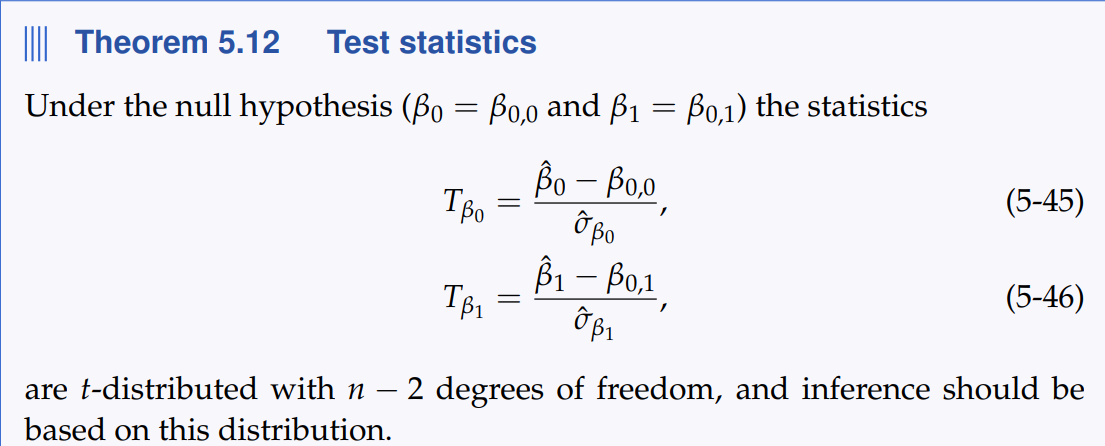
\includegraphics{images/paste-D0E70AC5.png}

Vi tester:~

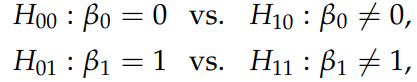
\includegraphics{images/paste-F94E956B.png}

\begin{Shaded}
\begin{Highlighting}[]
\NormalTok{B0 }\OtherTok{\textless{}{-}} \FunctionTok{coef}\NormalTok{(fit)[}\StringTok{"(Intercept)"}\NormalTok{]}
\NormalTok{B1 }\OtherTok{\textless{}{-}} \FunctionTok{coef}\NormalTok{(fit)[}\DecValTok{2}\NormalTok{]}
\end{Highlighting}
\end{Shaded}


\end{document}
